\textbf{Beispiel 1}\\ \\
a)\\ \\
Die gesuchte Masse lautet
\begin{align*}
	m_2 &= \int_{0}^{T}\int_{0}^{L}\int_{0}^{\tan(\alpha)x}\rho_2 \,\, \text{d}y\text{d}x\text{d}z \\
	&= \int_{0}^{T}\int_{0}^{L}\rho_2\tan(\alpha)x \,\, \text{d}x\text{d}z \\
	&= \int_{0}^{T}\rho_2\tan(\alpha)\frac{L^2}{2} \,\, \text{d}z \\
	&= \frac{1}{2}\rho_2L^2T\tan(\alpha)
\end{align*}
Der Schwerpunkt lautet
\begin{align*}
	s_x &= \frac{\int_{0}^{T}\int_{0}^{L}\int_{0}^{\tan(\alpha)x}x\rho_2 \,\, \text{d}y\text{d}x\text{d}z}{m_2} \\
	    &= \frac{\frac{1}{3}\rho_2L^2T\tan(\alpha)}{\frac{1}{2}\rho_2L^2T\tan(\alpha)} = \frac{2}{3}L \\ \\
	s_y &= \frac{\int_{0}^{T}\int_{0}^{L}\int_{0}^{\tan(\alpha)x}y\rho_2 \,\, \text{d}y\text{d}x\text{d}z}{m_2} \\
	    &= \frac{\frac{1}{2}\frac{1}{3}\rho_2L^3T\tan^2(\alpha)}{\frac{1}{2}\rho_2L^2T\tan(\alpha)} = \frac{1}{3}\tan(\alpha)L
\end{align*}
b)\\ \\
Freigeschnittene Körper:
\begin{figure}[h]
	\centering
	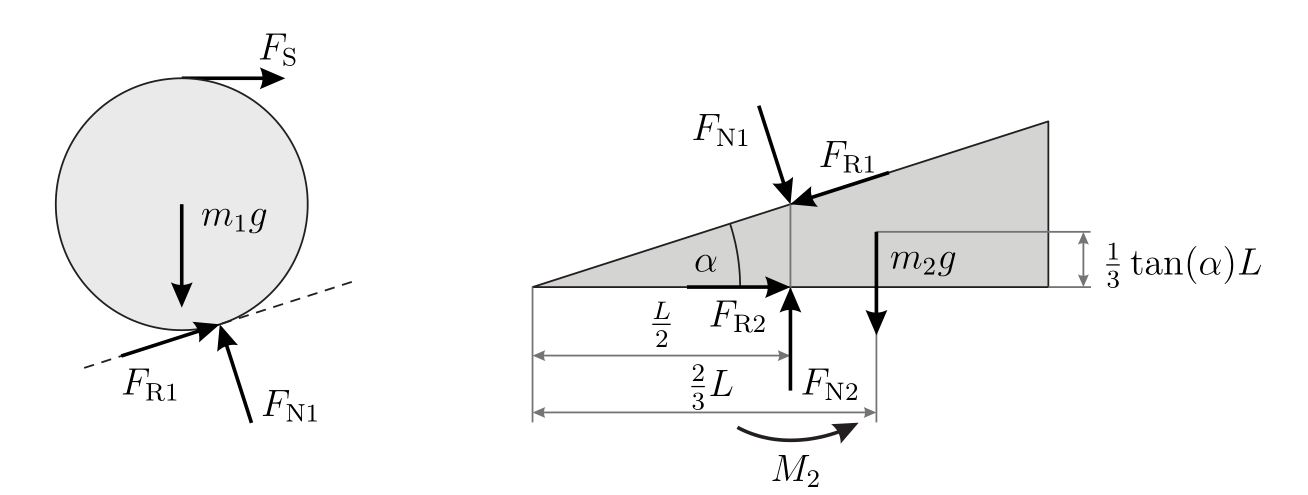
\includegraphics[width= 12.5cm]{tikz/16_03_2018_1b}
\end{figure}
\newpage
\noindent
c)\\ \\
Die geforderten Gleichgewichtsgleichungen lauten für die Walze
\begin{align*}
	\textbf{e}_x &: F_{R1}\cos(\alpha) + F_s - F_{N1}\sin(\alpha)\\
	\textbf{e}_y &: -m_1g + F_{R1}\sin(\alpha) + F_{N1}\cos(\alpha)\\
	\textbf{e}_z &: -rF_S + rF_{R1}
\end{align*}
und den Keil
\begin{align*}
	\textbf{e}_x &: F_{R2} - F_{R1}\cos(\alpha) + F_{N1}\sin(\alpha)\\
	\textbf{e}_y &: F_{N2} - m_2g - F_{R1}\sin(\alpha) - F_{N1}\cos(\alpha)
\end{align*}
d)\\ \\
Durch umformen dieser Gleichungen folgt für die gesuchten Kräfte
\begin{align*}
	F_{N1} &= m_1g & F_{N2} &= m_1g + m_2g \\
	F_{R1} &= m_1g\frac{\sin(\alpha)}{1+\cos(\alpha)} & F_{R2} &= -m_1g\frac{\sin(\alpha)}{1+\cos(\alpha)} \\
	F_S &= m_1g\frac{\sin(\alpha)}{1+\cos(\alpha)}
\end{align*}
e)\\ \\
Da es sich um Haftreibung handelt muss für Haftreibungskoeffizienten
\[
	\mu_1 > \frac{F_{R1}}{F_{N1}}, \quad \mu_2 > \frac{F_{R2}}{F_{N2}}
\]